
\section{\systemfull{} (\system{})}
\label{sec:method}

Overall architecture and dataflow within \system{} is shown in \reffig{fig:pipeline}. We describe each of the components in the sections below.

\subsection{Data Preprocessing}
\label{sec:dataextraction}

With Google API, we use RESTful requests to get web search links. Given the primary entity (PE), documents relevant to it are downloaded by issuing queries against Google. In order to make the query specific, especially in case of ambiguous entities, 
a few keywords are also added to the query. For the experiments in this paper, the category is used as the keyword. For example, for the entity \textit{Albert Einstein} from the \textit{scientist}
category, the query will be \textit{"Albert Einstein scientist"}. 
Whenever available, any attribute(s) of the entity is also included as keyword. Since our method is an unsupervised way of expanding the KB, we keep the input from the user to a very minimal extent.   
Entity linking service is used to find the wikipedia page of the primary Entity. This helps us in disambiguating the similar entities and rejecting the wikipedia links of disambiguous entities.
On an avg.top 20 documents returned by the search engine are downloaded and processed further. Number of documents are restricted by the Google API query limits.
Text is extracted from the raw downloaded html documents using regex patters, HTML tag matching, and by using
the Boilerpipe tool\footnote{Boilerpipe: http://code.google.com/p/boilerpipe}.

%The source of data is web documents and searches are made specific to primary entity. Key words related to primary entity are used while querying so as to get more relevant and useful  documents. The key words can be either user specified or domain name to which the entity belongs to. In our work, for most of the experiments domain name was used as the key word. One more approach tried was getting relevant words from knowledge bases. Freebase id of the entity is used to get the attributes from freebase. For e.g. attributes like place and date of birth, religion etc are listed for person category.  These attributes acts as key words and improves the search results.
%Web page contents are downloaded, cleaned and dumped to local system. The processing of the raw data is done using regex pattern matching, HTML tag matching and the Boiler-pipe, a tool to extract text from web documents.

\subsection{Triple Extraction and Processing}
\label{sec:tripleextraction}
Text of each document obtained in the previous step is processed through the Stanford CoreNLP toolkit\cite{manning2014stanford}. Stanford CoreNLP provides a set of natural language analysis tools. It can give the base forms of words, their parts of speech, whether they are names of companies, people, etc., 
normalize dates, times, and numeric quantities, and mark up the structure of sentences in terms of phrases and word dependencies, indicate which noun phrases refer to the same entities. 
We use the sentence tokenization, coreference resolution, NER and POS tags and dependency parsing features of the CoreNLP toolkit.
Sentences without resolving coreference are then passed through OpenIEv4 \footnote{OpenIEv4: http://knowitall.github.io/openie/} to extract  \textit{(noun phrase, predicate,noun phrase)} triples. 
Coref resolution is performed on these triples using the output of CoreNLP toolkit. 
Multiple and overlapping triples from the sentence was permitted. Length filter is applied on the noun phrase and the predicate of the triple extracted. This eliminates
triples whose predicate is more than 6 tokens and noun phrase more than 8 tokens.\\
The above process of representing sentence in a triple form is quite noisy. We loose lot of information when a big sentence is break down to a triple. 
For e.g. A sentence explaining bombing incident may contain place, time, victim, culprit, but OpenIE breaks it into many triples, each of which on their own does not describe the event completely.
Example given below explains the few possibilities of noise induction.\\
Sentence:\textit{In 1940 Albert Einstein renounced his German nationality law for a second time and became a U.S. Citizenship.}\\
OpenIE Extractions:
\begin{itemize}
\item{0.91747 :(Albert Einstein;renounced;his German nationality law)}
\item{0.91747 :(Albert Einstein;renounced;for a second time)}
\item{0.91747 :(Albert Einstein;renounced;In 1940)}
\item{0.95421 :(Albert Einstein;became;a U.S. Citizenship)}
\item{0.95421 :(Albert Einstein;became;In 1940)}
\end{itemize}

Third and the last triple are capturing only time and hence miss the context. Second triple is a not very informative.

\textbf{Entity Disambiguation and Linking:} It is the task of determining the identity of entities mentioned in text.
Named entity mentions can be highly ambiguous, any entity linking method must address this inherent ambiguity, 
We use dexter entity linking system which finds and mapps the entity mentions in the text to wikipedia page titles. 
This phase helps in clustering the different mentions of the same entity.

\textbf{Extraction of Entity from Noun Phrase:}
Even after applying length filter, long noun phrases may not represent a real world entity. Consider the example given below,\\
Sentence:\textit{Soon after their divorce, Albert Einstein married his cousin Elsa.}
\begin{itemize}
\item{0.91746 :(Albert Einstein;married;his cousin Elsa)}
\item{0.91746 :(Albert Einstein;married;Soon after their divorce)}
\end{itemize}
OPenIE extraction has marked \textit{his cousin Elsa} as the Entity-2, but we would like to have \textit{haswife(Albert Einstein,Elsa)} as the instance of the KB. Now the challenge is how to 
select only "Elsa" from "his cousin Elsa". We term this as the task of obtaining entity from noun phrases.
One more challenge here is to filter out the second triple because \textit{haswife(Albert Einstein, divorce)} is an erroneous tuple.\\

To address both the task of obtaining entity from noun phrase and rejecting the wrong triples, we use a scoring mechanism. Scoring mechanism is based on the POS tag patterns of the entities present in wiki dump[ref??]

POS tag patterns of entities from wikipedia dump are mined and stored along with their counts. POS tag of any given noun phrase is matched with the existing POS tag patterns and the best match from phrase is selected as Entity-2.
Frequency of the matched POS tag pattern, ratio of the length of Entity-2 to length of noun phrase and openIE score is used to calculate triple score.\\

Triple Score = Frequency of POS tag * (number of words in Entity-2/Number od words in noun phrase) * OpenIE score\\

%\reminder{MGH: Add example or few top and bottom ranked entities}

% Sentence:\textit{Albert Einstein himself had always opposed long and horrifying war.}\\
% OpenIE Extractions:\\
% \begin{itemize}
% \item{0.92564: (Albert Einstein;had opposed;long and horrifying war)}
% \item{0.92564: (Albert Einstein;had opposed;always)}
% \end{itemize}
% Replace "long and horrifying war" to "war"
% Reject the second triple\\



%Raw data from the web contains many indirect references, so it is also important to address the co-reference resolution problem here. 
%Indirect references can be either pronouns, adjectives or some variations of the entity string. The Stanford co-reference resolution tool is used for sentence tokenizing and coreference resolution. The dependency tree structure is used to extract the entity when the output entity of the Stanford CoreNLP was greater than certain threshold. The sentences formed are used as input to openIE for triple extraction.\\
%OpenIE is a tool to extract triples from the sentences. These output triples have a \textit{subject predicate object} format. 
%The extractions from the OpenIE have the score mentioning the correctness of the extraction. Each sentence will have multiple extractions with different confident scores. 
%We consider multiple extractions from the same sentence. 2 extractions for the sentence \textit{Modi sell tea at vadanagar railway station} were 
%\textit{(Modi, sell, tea)} and \textit{(Modi, sell tea at, Vadanagar railway station)}. Considering both the extractions helps us to find the new entity \textit{vadanagar railway station}.
%Constraints are imposed on the length of the phrases which are acting as relation and entity2. This eliminates the many such phrases which are extracted from OpenIE, 
%but are not representing a real time entity or relation.  

%\subsection{Clustering entities and relations}
\subsection{Noun and Relation Phrase Normalization}
\label{sec:normalization}

Noun phrases (NPs) and relation phrases obtained from the previous step are normalized (or canonicalized) in this step. Canopy clustering technique as proposed in \cite{canopy} was 
used for noun phrase as well relation phrase clustering. 
Initial clustering is done over the \textit{unlinked} noun phrases in the triples. Please note that since we are working in an entity-centric manner, one of the two NPs present in the triple is already connected to the knowledge graph, and hence is considered \textit{linked}. 
To cluster noun phrases, we first construct canopies corresponding to each word in the noun phrase. For example, 
for noun phrase \textit{Albert Einstein}, we create two canopies, viz., a canopy for  \textit{Albert} and another canopy for  \textit{Einstein}, and add \textit{Albert Einstein} to both canopies. 
Grouping of noun phrases inside the canopy is the next step of clustering phase.
Noun phrase similarity is calculated based on  similarity of words in the noun phrases. 
Word similarity is either direct string matching or Gensim similarity score\footnote{https://github.com/piskvorky/gensim/}, which internally uses word2vec
embeddings \cite{mikolov2013distributed}. After calculating pairwise similarity of noun phrases, hierarchical clustering is carried out to group noun phrases inside each canopy. 
A threshold score is used to stop hierarchical clustering. At the end of this process, we have canopies and groups of noun phrases inside them. 
A noun phrase can be in more than one canopy, hence those groups across canopies are merged if the similarity is greater than certain threshold. After this, each group will contain facts which have similar noun phrases and different (or same) relation phrase.
Again the facts are clustered based on the similarity of the relation phrase. Relation phrase similarity calculation step resembles the one used for noun phrases as described above.

After this triple clustering step, the best representative triple from each cluster is selected based on a few rules. We consider the structure of POS tags in noun phrases of a triple as one of the criteria. Secondly, if both noun phrases in the triple are linked to the knowledge graph, then it makes the triple more likely to become a representative tuple of the cluster. Also, if the NPs present in the triple are frequent in the cluster, then it makes the corresponding triple more like to become a representative.

%We consider the structure of POS tags of the noun phrase as one of criteria for selection. %The entities that appear in the document follow some common structure like noun followed by noun or adjective followed by noun. 
%Next criteria is the presence of entity in the triple. The entity2 of the triple if it has a freebase id then it is an evidence that the triple extracted is a useful fact. 
%We also consider the frequency of the noun phrase in the cluster(num of facts having the noun phrase as entity2) for selection.

%The triple extractions from the previous step are clustered in this phase. As the aim is to find (relation, entity) pair for the primary entity from the extractions, grouping is done so that 
%similar extractions lie in a same set. The initial ideas of canopy clustering \cite{canopy} is used for entity and relation cluster. 
%To cluster entities, we first construct canopies. 
%Each word in the entity is either added to a canopy or new canopy is constructed if not present. For entity say \textit{Albert Einstein}, we create 2 canopies namely canopy \textit{Albert} and canopy 
%\textit{Einstein}. Each will have
%the entity \textit{Albert Einstein}. Since the entities inside each canopy share a word, the probability of they being similar is high. Next step is to find the similar entities inside each canopy and group them.
%To find the similarity between two entities we define pair wise similarity function. This function considers each phrase or the entity as the bag of words.
%The string and freebase id matching techniques are used to find the similar entities. When the words don’t match, the gensim model is used to calculate the similarity between the words.
%For e.g., if the entity one has 3 words \textit{w1, w2, w3} and entity two has 2 words \textit{x1, x2}, similarity is calculated as follows, For each word ‘w’ in entity one, find the best
%match in entity 2. If string match of w and x is true, then similarity score is 1, else use the similarity score returned by gensim similarity function. Add all these word wise similarity
%score and divide it by the number of words in the phrase. 
%After the similarity calculation, grouping of entities is done in the following way. Inside every canopy, group those 2 entities which are mutually close to each other into one set. An hierarchical clustering 
%is carried until the similarity is greater than threshold. Merging happens across canopies also. So after the clustering phase, each set will have triples where entities participating are similar. 
%The similarity of relations within each set is calculated for final grouping of the triples. The bag of words and gensim is used again to find relation similarity. After final grouping, each set will have triples which convey the same fact. \\

%\subsection{Entity and Relation Normalization}
%After grouping similar extractions, the best possible candidate from the group is selected based on few rules. 
%The aim of selecting the extraction and cleaning the entity is to represent the extraction as a knowledge fact. This helps us to map the fact to existing knowledge bases. 
%The pos tag structure of entities are studied and the filters (defined in Katz filter) are used to extract the best possible entity structure from the phrase.

%\subsection{Matching extraction to NELL}
\subsection{Integrating with Knowledge Graph OR Relation Mapping}
\label{sec:rel-map}
\subsubsection{ Distance supervision}
\cite{mintz2009distant} proposed distant supervision for the first time in 2009. Their approach uses Freebase, a large semantic database to provide distant supervision for relation extraction. The algorithm
assumes that any sentence containing two entities expresses relation between those two entities as given in freebase.
Unlike supervised setting, this approach is noisy, but can learn well due to large number of examples. 
The algorithm depends on a database for it’s relation instances, and therefore does not suffer from domain-dependence or overfitting.\\
We use distance supervision to map the relation in a triple to a nell-relation. 
The distant supervision assumption is that if two entities participate in a relation, any sentence that contains those two entities might express that relation.
With the above assumption, we generate training data for relation mapping using the instances from NELL. Detailed procedure for generating positive and negative training 
is described below.
Web data is the source of distance supervision for both negative and positive training samples.
For the task of relation mapping, we have hand picked 110 nell-relations.
We are using the high confident nell instances and consider them as the true lables for all of the selected nell-relations.
For each nell-relation we get 100 to 500 instances of the form \{Entity-1:Entity-1-type, Entity-2:Entity-2-type\}


For positive training samples, we take instance pairs (Entity-1,Entity-2) and using the initial part of the pipeline[??], we collect
sentences from web pages. We use wildcard character '*' between entities ("Entity-1 * Entity-2") in the Google search to get more accurate sentences. These sentences contains both entities and hence represent the relation.

Even for negative training samples, we consider same set of nell relations. The generation of instances differs from positive data collection. We take Entity-1 from the instance pair and
Entity-2-Neg is collected as follows, select an entity which has type same as Entity-2 and "Entity-1 nell-relation Entity-2-neg" is not present in NELL.

Example, for nell relation 'personborninlocation', NELL instance pair (Obama:person, Honolulu:location)\\
Sentences selected as positive training example are\\
\begin{itemize}
 \item Barack Hussein Obama, born in Honolulu on August 4, 1961.\\
 \item However, a view of the various homes where Obama dwelled in Honolulu reveals a broader, diversified beginning.\\
\end{itemize}
Examples for negative training.\\
\begin{itemize}
 \item Obama Pokes Fun at Friends and Enemies at dinner held in Washington.\\
 \item Obama walks to stage at rally in Washington.\\
\end{itemize}

There is always a noise factor associated with distance supervision and it affects the accuracy of the system. 

\subsubsection{CNN for Relation Mapping:}
High level architecture of the CNN is shown in \reffig{fig:cnn}
\begin{figure*}[!htbp]
\begin{center}
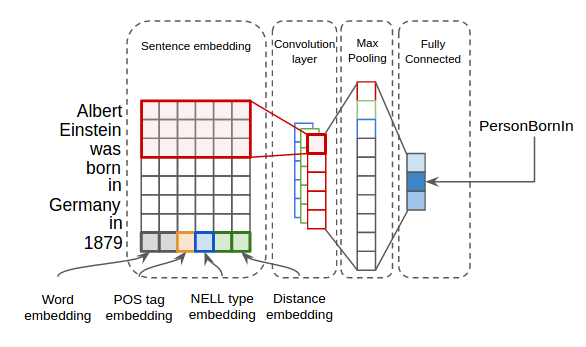
\includegraphics[scale= 1]{images/CNN.png}
\end{center}
\caption{CNN for relation mapping. See \refsec{sec:rel-map} for details.}
\label{fig:cnn}
\end{figure*}
For relation linking, the distantly supervised training data is used to train a classification model. Given an instance, which consists of a plain text sentence, an entity pair, and the NELL type of the entities, the model generates a probability distribution over the candidate relations. 

The classification model used is a Convolutional Neural Network (CNN) following \cite{kim:2014}. In this model, the input instance is represented by an $ n \times d$ \textit{image}, which is then fed through a CNN. Two filters (of height 1 and 2) are used in a single convolution layer, followed by a max-pooling layer. These are 1D (temporal) convolutions, and therefore the width of the filter is equal to the width of the image. The height, therefore, is analogous to the size of a context window around tokens in a sentence.

To convert the raw text into an input image, the following features are used. Each feature is embedded using a matrix of parameters that is learned as part of the training process.

\begin{itemize}
\item Word features: word ids are embedded using an embedding matrix that is initialized using Glove \cite{pennington2014glove} vectors. 
\item POS tags: Generated using CoreNLP
\item NELL type information: Generated using ???
\item Position features: From \cite{zeng:2014}, these features are integers that represent the relative distance of each token from an anchor entity (see Fig.). Two such features are generated, one for each entity in the entity pair. These features are useful in incorporating temporal information about word-ordering into the input, which otherwise a CNN is agnostic to.
\end{itemize}

$d$ is therefore $d_{word} + d_{pos-tag} + d_{NELL-type} + 2\times d_{position})$. $d_{word}$ is set to 300, while all the other embedding matrices are chosen do be 50 dimensional. The number of filters used is 256.

\subsubsection{Relatiom Mapping Using Extraction Patterns}
The set of normalized triples from the previous step are linked with the Knowledge Graph, whenever possible, in this step.
Metadata for each relation in NELL has a set of verb phrases, which capture the variation of the nell-relation in free text.
The similarity of words in triple to avg similarity of words in the extraction pattern is used for relation mapping.
GloVe vector representation of words is the key behind calculating the similarity. GloVe is an unsupervised learning algorithm for obtaining vector representations for words. 
Training is performed on aggregated global word-word co-occurrence statistics from a corpus. Each word is represented as a vector of dimension 300.
The algorithm \ref{alg:RMalgorithm} describes all the steps of relation mapping.
Whenever this extraaction pattern based mapping is not possible, then the predicate is listed as a new relation, and the
corresponding triple marked to belong to either NR-KE or NR-NE extraction class, depending on whether the target entity is already present in the KG or not.

\begin{algorithm}

\caption{Relation Mapping with Extraction Patterns and Glove Vectors}

\label{alg:RMalgorithm}

\begin{algorithmic}[1]

\Procedure{Relation Mapping}{}

\State Triple: \textit{Entity-1,relation,Entity-2}
\State get entity type (\textit{Entity-1-Type,Entity-2-Type}) using NELL Json API

\State relation vector (RV) = initialise 0-vector of length 300
\For{each word in relation}
\State RV = RV + GloVe(word)
\EndFor
\State RV = RV/number of words in relation

\State S = Set(nell-relations which satisy type constraints)
\For{each nell-relation in S}
\State P=Extraction patterns for nell-relation
\For{each extraction-pattern in P}
\State EPV = initialise zero vector
\For{each word in extraction pattern}
\State EPV = EPV + GloVe(word)
\EndFor
\State EPV = EPV/number of words in extraction pattern
\EndFor
\State similarity = cosineSimilarity(RV,EPV)
\EndFor
\State Mapped Relation = relation with maximum similarity score
\EndProcedure
\end{algorithmic}

\end{algorithm}
%%%
%%%
% The set of normalized triples from the previous step are linked with the Knowledge Graph, whenever possible, in this step. For a given normalized triple, 
% following steps are performed as part of linking. First, category of each noun phrase in the triple is obtained based on string matching. In case of no match, refinements like dropping of adjectives, considering only noun phrases are done to for rematching. 
% Now, the relation phrase is mapped to an existing predicate in the KG based on the extraction patterns in the metadata of the target relation (e.g., NELL and many other KGs have such metadata available).
% Candidate predicates are chosen from the above mapped predicates based on category signature of the two noun phrases (i.e. entity1 and entity2). This is possible since the all the predicates in NELL have the type signature defined in the metadata.
% Frequency of the relation phrase in the metadata is used as a criteria to select a candidate from multiple predicates.
% If such category-signature based mapping is not possible, then the predicate is listed as a new relation, and the
% corresponding triple marked to belong to either NR-KE or NE-NE extraction class, depending on whether the target entity is already present in the KG or not.
%%%
%%%

%Problem with openIE kind of fact extractions is that, they can be highly disambiguated. Both entity and relation phrase of the extraction contribute to ambiguity. 
%For e.g. consider a fact Josephine C. Cohen  married  Mollie Levy,  
%The other occurrences of Josephine C Cohen like Cohen, J C Cohen and other relation phrases for married can husband of. 
%These different combination can give rise to different representation for the same fact.
%NELL has metadata for each relation. E.g. \textit{has spouse} is a NELL relation which is mapped to relation phrases like married, husband of, wife of etc. 
%This metadata about the relations is used to map the relation phrase in the extraction to a NELL-relation. It is also important to know the
%types of the entities that are participating with the relation to reduce the ambiguity of the relation mapping. 
%To get the types of the entities and classify the extraction, entities are mapped to NELL Some heuristics are made while matching entities to NELL. 
%Following are the steps followed while matching an entity to NELL. If the exact match of the entity is found then get the type signature of the entity. 
%Remove phrases like Mr. Mrs. Dr. or adjectives from the entity in the extracted fact and then match it to NELL. 

%So for a given fact, following steps are done as a part of mapping. Get the type signature of the entities in the fact. map the relation phrase to NELL-relation 
%based on the type signature of the entities. Mapping a fact to NELL can be either hit or a miss. We call it a hit when both the relation and second entity
%(we know that primary entity is present in NELL ) is present in the knowledge base. Even though both the entity and relation exists in knowledge graph, there may not be an edge connecting those two. 
%So we classify hit into new and existing fact based on the presence of the edge. A miss occurs when either relation or a second entity is absent in the knowledge base. 

